\documentclass[12pt, a4paper]{article}

\usepackage[T1]{fontenc}
\usepackage[utf8]{inputenc}
\usepackage[english, polish]{babel}
\usepackage{polski}
\usepackage{graphicx}
\usepackage[export]{adjustbox}
\usepackage{amsmath}
\usepackage{pdfpages}
\usepackage{enumerate}
\usepackage{siunitx}
\usepackage{geometry}
\usepackage{float}


\begin{titlepage}
\centering
\author{
	\\ Maria Konieczko
	\\ Alicja Poturała
	\\ Marcin Dolicher
	\\
	\\ AIR Semestr V
}
\title{	
    DCS i SCADA \\
	Sprawozdanie z Projektu I		
}


\date{}
\end{titlepage}

\newgeometry{tmargin=3cm, bmargin=2cm, lmargin=2.5cm, rmargin=2.5cm}
\graphicspath{{../images/}}

\begin{document}
\maketitle
\newpage
\tableofcontents

\newpage
\section{Zagadnienia i założenia projektowe}
Postawione przed nami zadanie polegało na zaprojektowaniu regulatora PID, który steruje obiektem grzewczym, w naszym przypadku będzie to grzałka. Na obiekt działają zakłócenia w postaci wiatru generowanego przez wiatrak. Punkt pracy jest ustawiony na $30 \%$ mocy grzałki co daje nam stałą temperaturę w okolicach \ang{38}. Projekt regulatora i testy dla obiektu (zmiana zakłóceń i wartości zadannej) zostały przeprowadzone przy użyciu programów dostarczonych przez firmę Ovation. Do zebrania odpowiedzi skokowej wykorzystane zostało oprogramowanie MATLAB. Charakterystyka obiektu odpowiadała obiektowi 1 na 1 plus 1 (1 wejście, 1 wyjście i 1 zakłócenie). Regulator miał za zadanie utrzymywać zadaną wartość dla grzałki przy zmiennych wartościach zakłóceń. Ocena jakości regulacji polega na obliczaniu błędu średniokwadratowego dla sygnału sterującego w porównaniu do wartości zadanej. Najlepszy regulator został wyłoniony na podstawie konkursu na ostatnich zajęciach. 
\section{Identyfikacja obiektu}

\section{Struktura}

\section{Strojenie PID}

\subsection{f) }
\begin{figure}[h!]
%\includegraphics[scale=0.55, center]{sciezka do pliku}
\end{figure}
\newpage
\section{Testowanie}
Ostatnim etapem było testowanie działania stworzonej pętli regulacji poprzez sprawdzenie reakcji na zmianę temperatury zadanej oraz zmianę wartości sygnału sterującego dla wentylatora. 

\subsection{Testowanie zmiany wartości zadanej temperatury}

\begin{figure}[H]
	\centering
	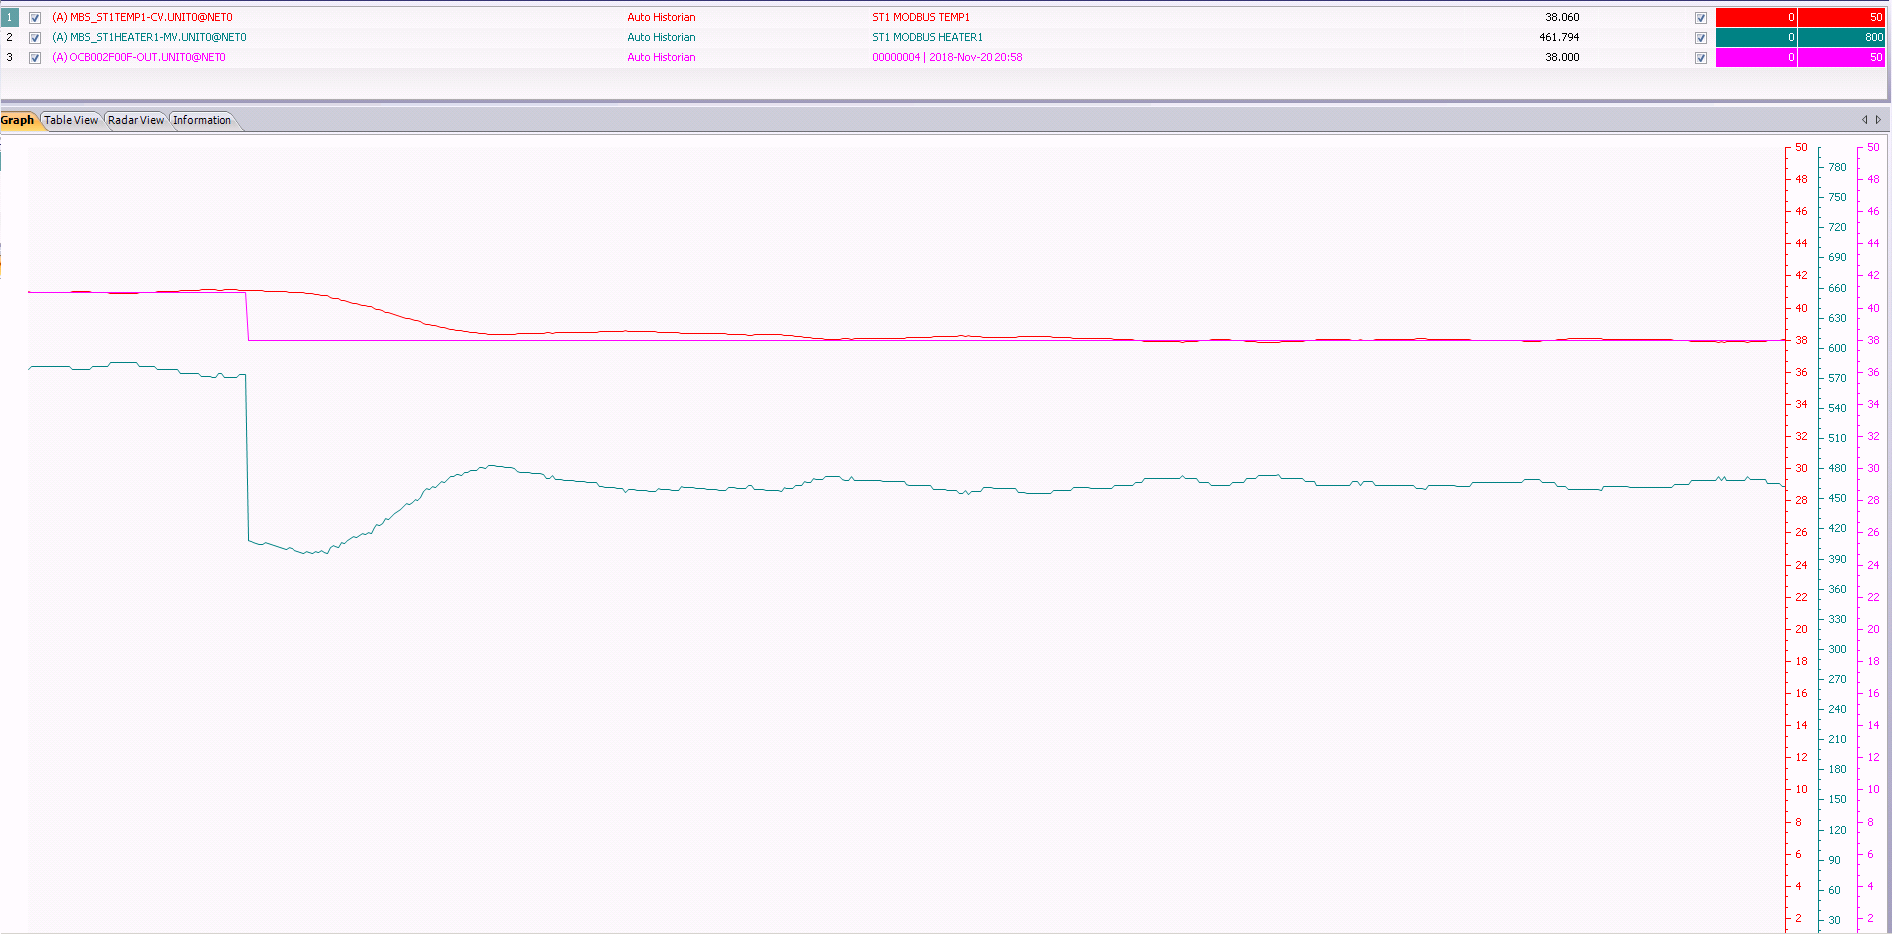
\includegraphics[width=0.9\linewidth]{SKOK_STEROWANIA}
	\caption{Wykres przebiegu sygnałów uzyskany podczas konkursu: czerwony - osiągnięta temperatura, różowy - wartość zadana temperatury, granatowy - sterowanie wentylator, morski - sterowanie  grzałki}
	\label{fig:SKOK_STEROWANIA}
\end{figure}
\begin{figure}[H]
	\centering
	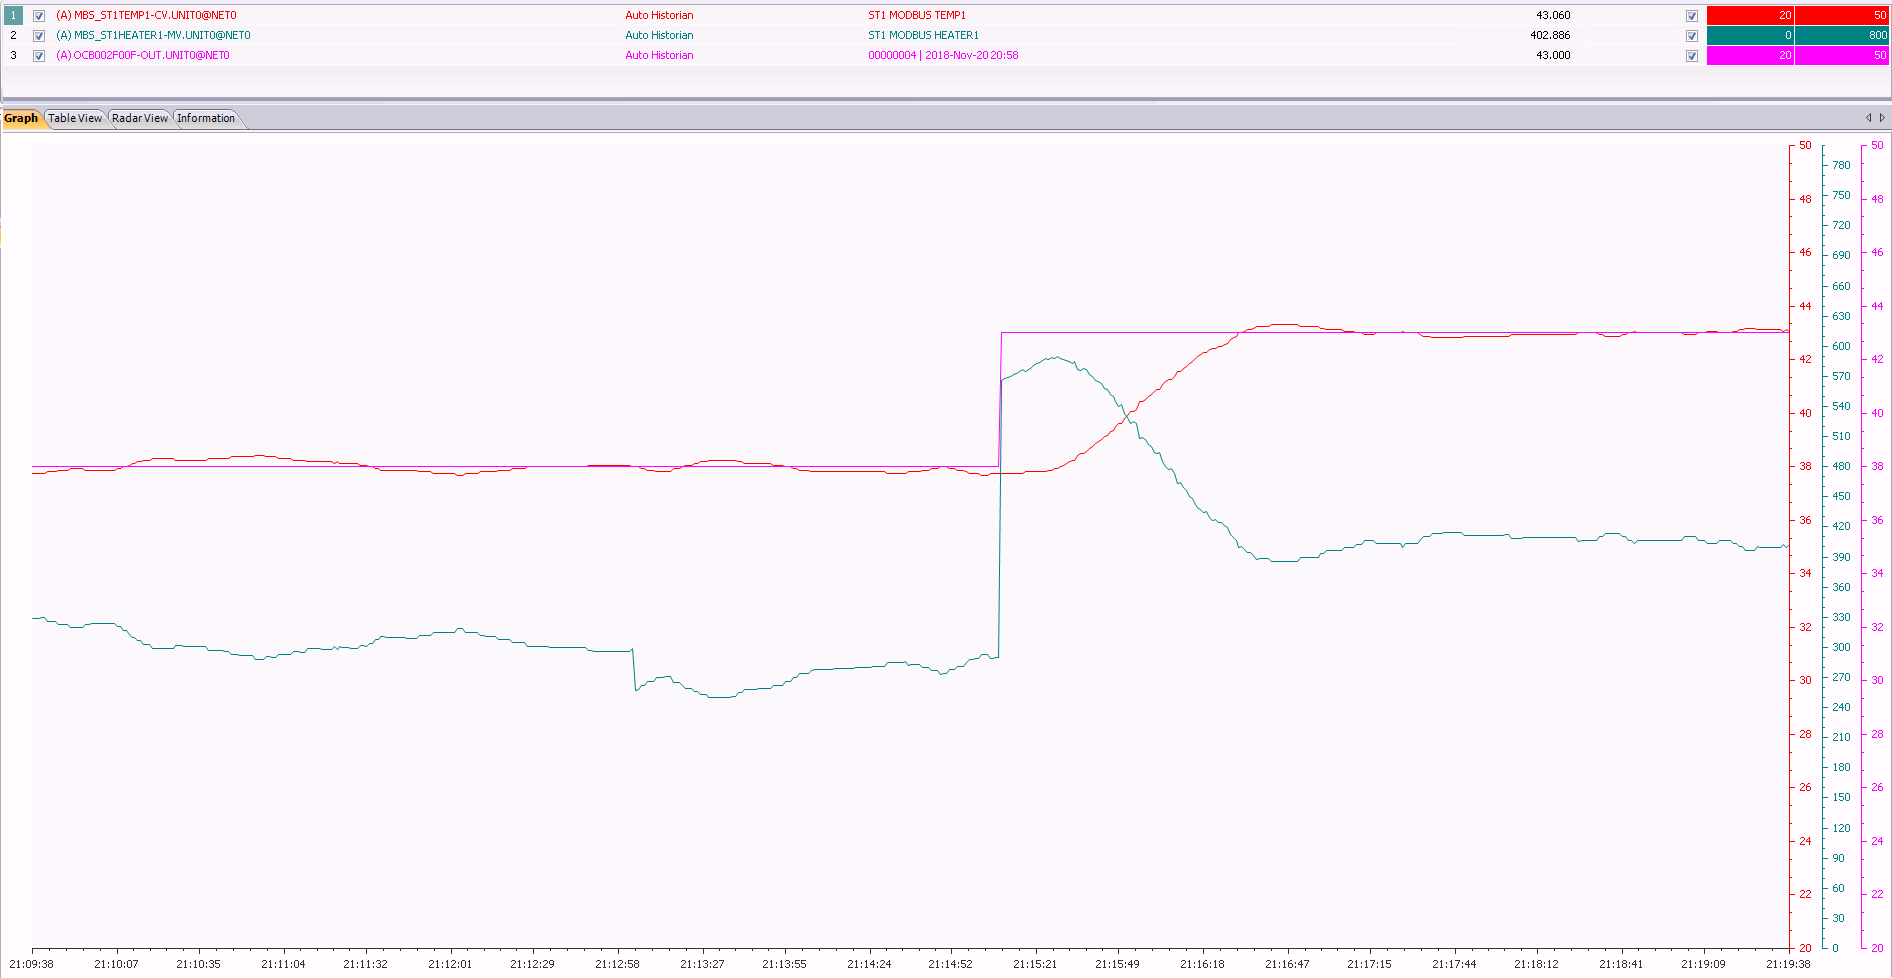
\includegraphics[width=0.9\linewidth]{sterowanie3843}
	\caption{Wykres przebiegu sygnałów uzyskany podczas konkursu: czerwony - osiągnięta temperatura, różowy - wartość zadana temperatury, granatowy - sterowanie wentylator, morski - sterowanie  grzałki}
	\label{fig:sterowanie3843}
\end{figure}
\begin{figure}[H]
	\centering
	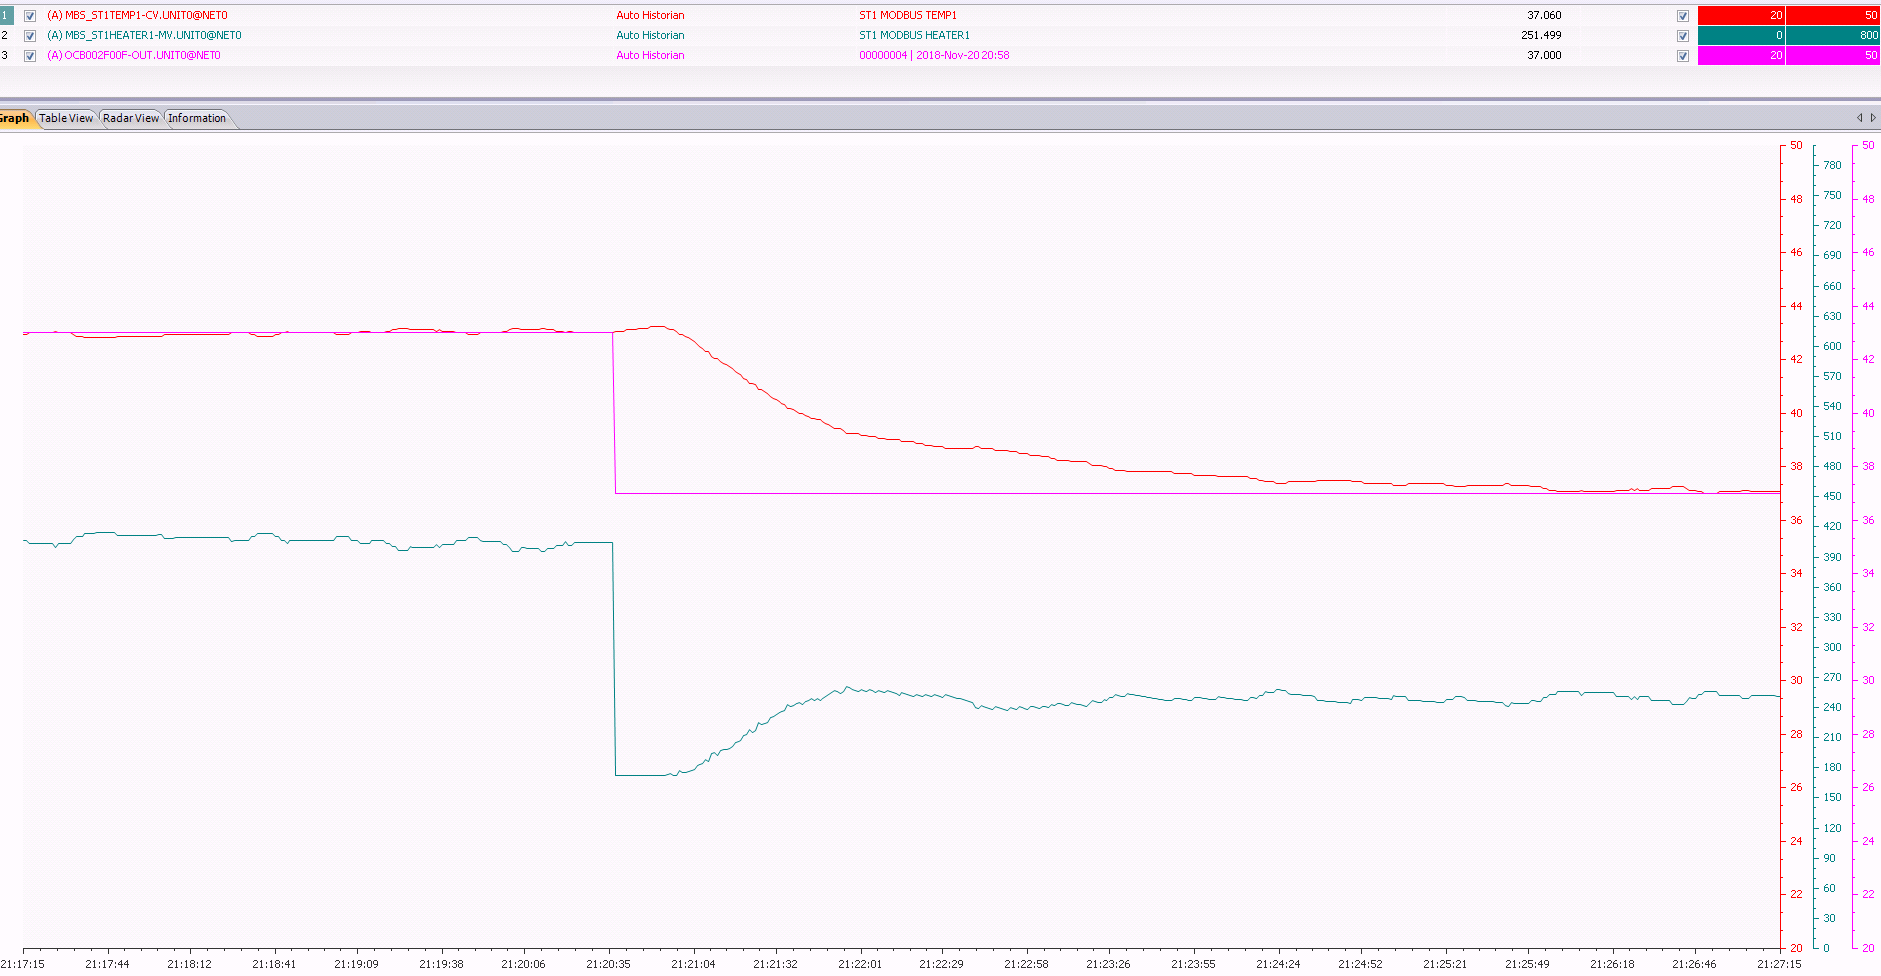
\includegraphics[width=0.9\linewidth]{sterowanie4337}
	\caption{Wykres przebiegu sygnałów uzyskany podczas konkursu: czerwony - osiągnięta temperatura, różowy - wartość zadana temperatury, granatowy - sterowanie wentylator, morski - sterowanie  grzałki}
	\label{fig:sterowanie4337}
\end{figure}
\begin{figure}[H]
	\centering
	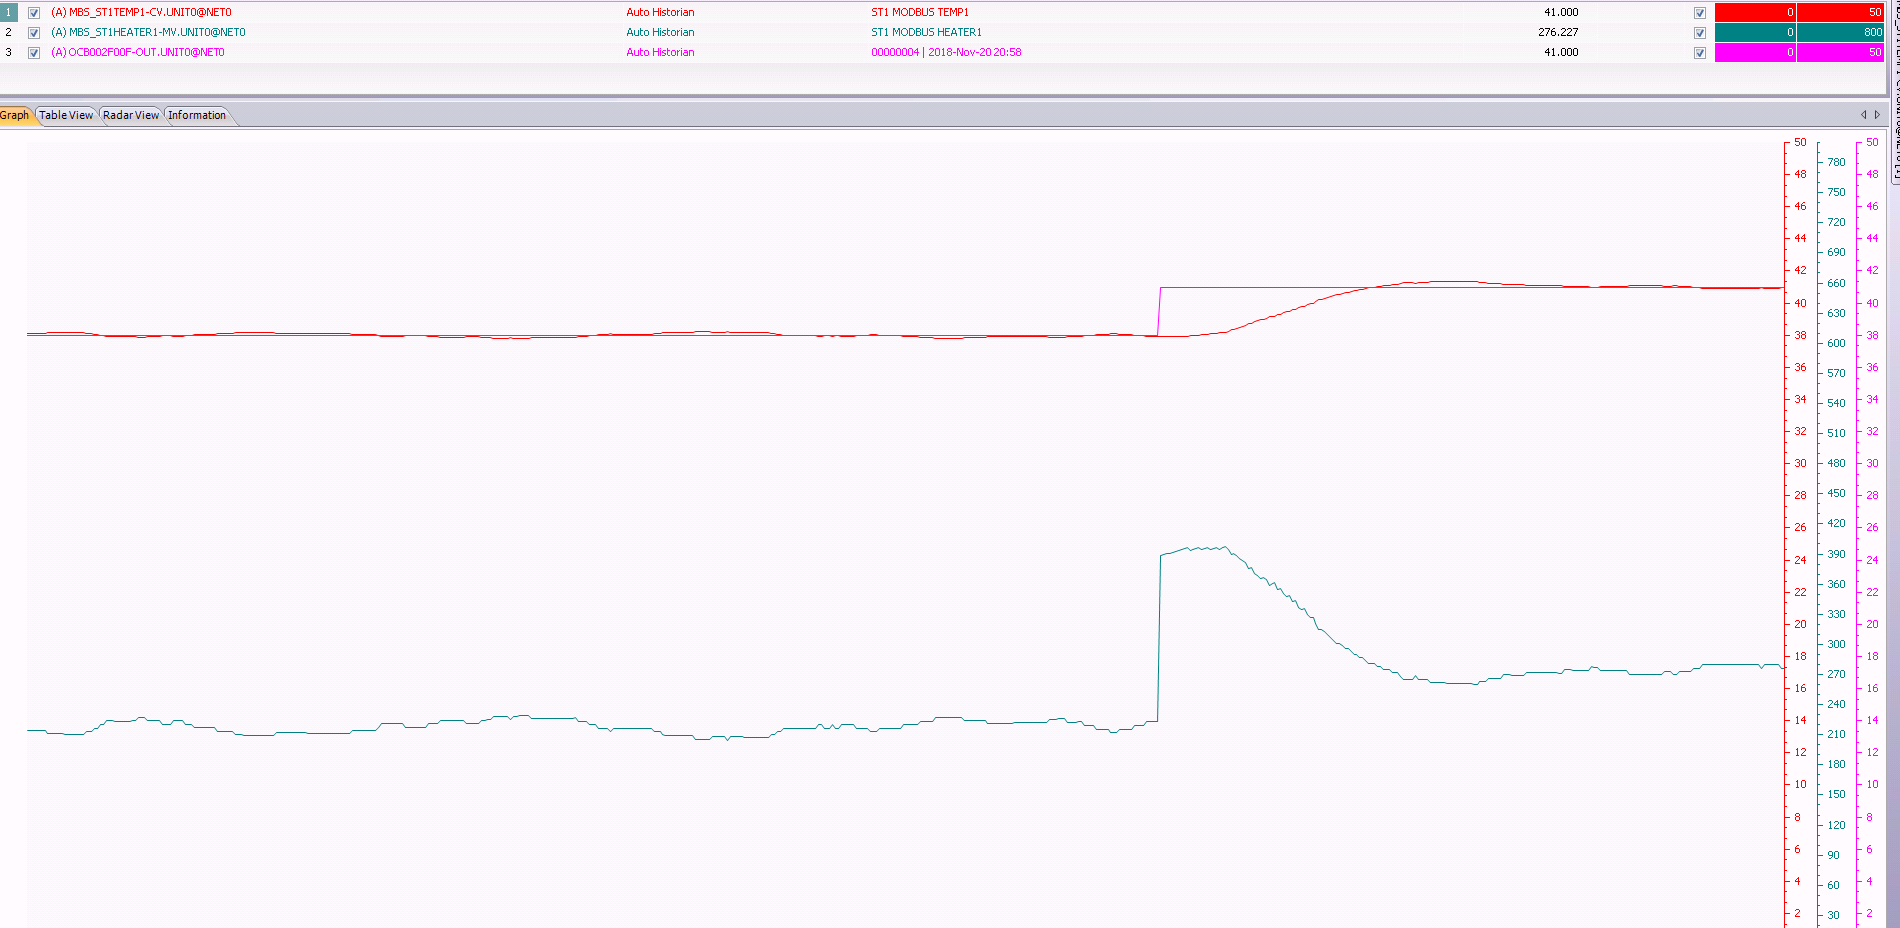
\includegraphics[width=0.9\linewidth]{wiatrak20temp3841}
	\caption{Wykres przebiegu sygnałów uzyskany podczas konkursu: czerwony - osiągnięta temperatura, różowy - wartość zadana temperatury, granatowy - sterowanie wentylator, morski - sterowanie  grzałki}
	\label{fig:wiatrak20temp3841}
\end{figure}

\subsection{Testowanie zmiany zakłócenia}


\subsection{Konkurs}
Ostatecznym sprawdzianem był udział w konkursie. Przebieg sygnałów uzyskanych podczas konkursu został ukazany na Rysunku \ref{fig:konkurs}. Podczas konkursu został wykonany skok wartości zadanej z $38^\circ$ na $44^\circ$. Po dojściu temperatury do zadanej wartości, zostało zmienione zakłócenie z 30 na 45. 

\begin{figure}[H]
	\centering
	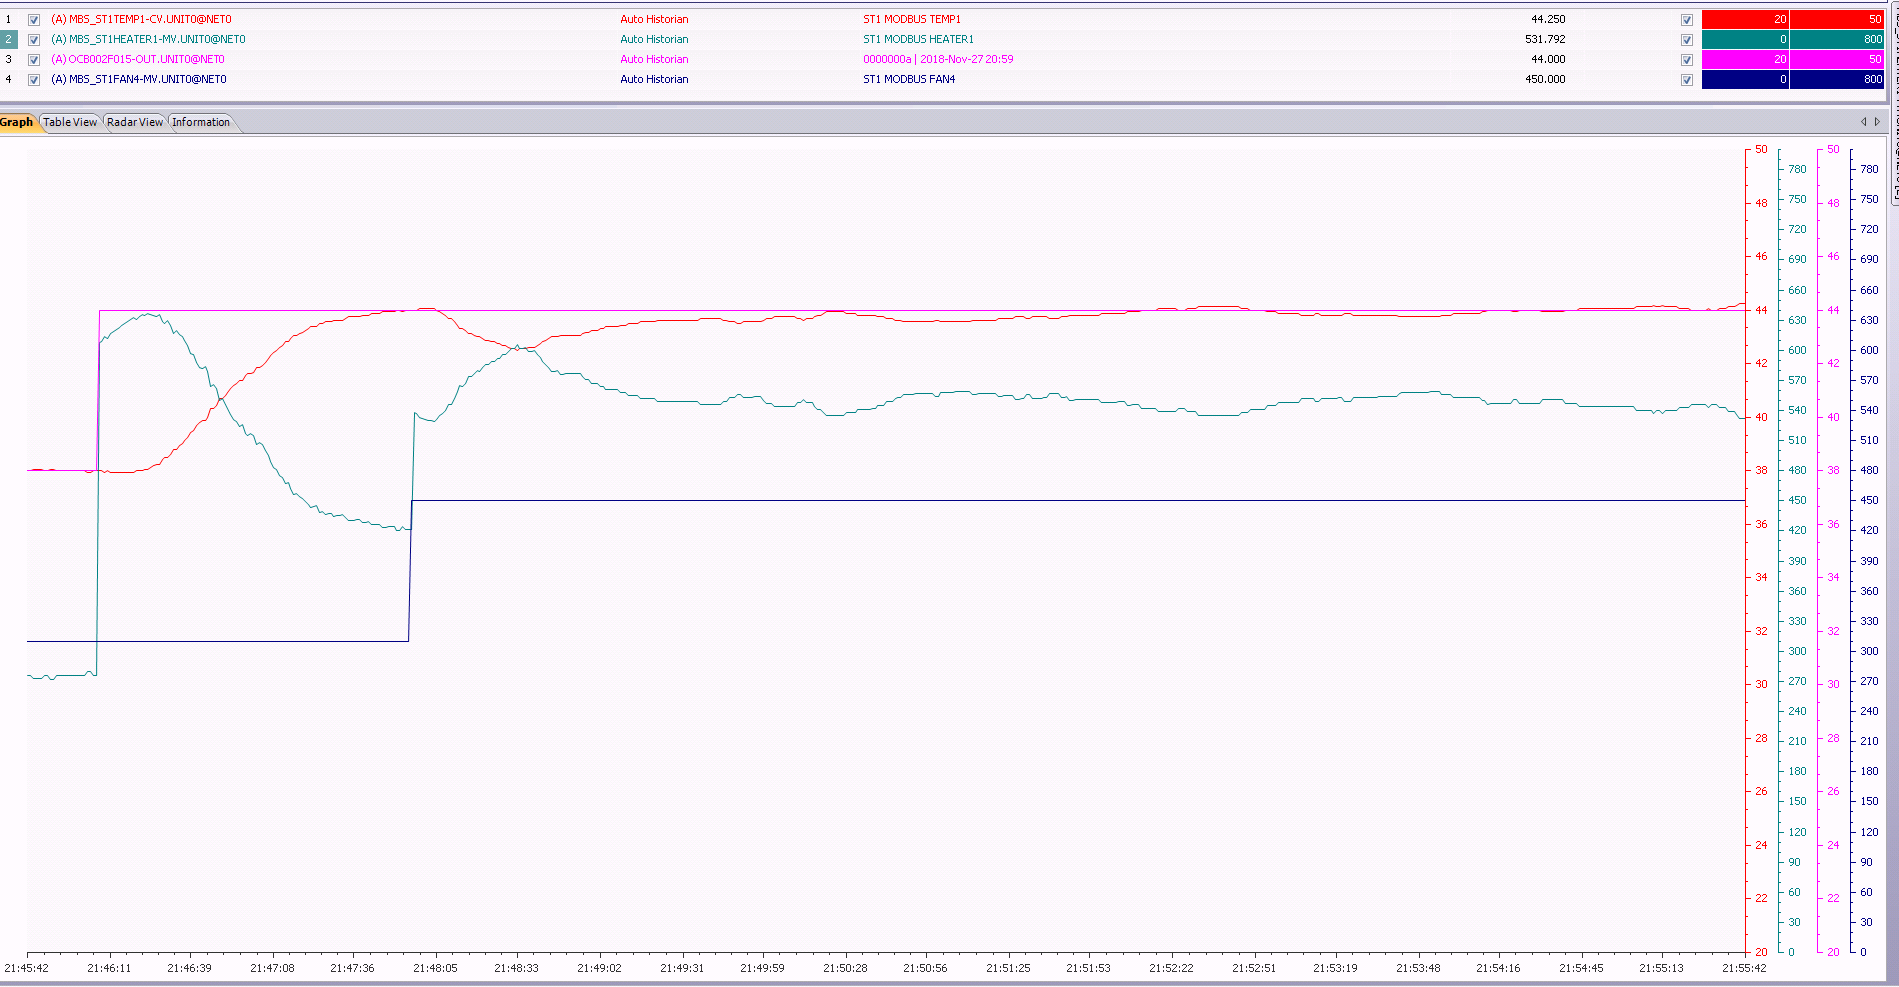
\includegraphics[width=0.9\linewidth]{konkurs}
	\caption{Wykres przebiegu sygnałów uzyskany podczas konkursu: czerwony - osiągnięta temperatura, różowy - wartość zadana temperatury, granatowy - sterowanie wentylator, morski - sterowanie  grzałki}
	\label{fig:konkurs}
\end{figure}

Przy zmianie wartości zadanej sygnał sterujący gwałtownie wzrósł, a potem zaczął maleć. Temperatura osiągnęła zadaną wartość po dwóch minutach. Zanim układ zdążył się ustabilizował zostało zmienione zakłócenie - wentylator zaczęł intensywniej pracować. Z tego powodu zmniejszyła się temperatura (nie da się całkowicie wyeliminować zakłócenia). Sygnał sterujący grzałką zwiększył swoją wartość, aby zniwelować zakłócenie. Następnie zaczął maleć, aby w końcu ustabilizować się na wartości większej niż przed skokiem zakłócenia - co jest logiczne z uwagi na to, że cały czas musi niwelować zwiększone sterowanie wentylatora. Temperatura osiagnęła spowrotem wartość zadaną

Jakość regulacji była oceniana jako suma błędów średniokwadratowych dla osiągniętej temperatury w porównaniu do wartości zadanej. Układ poradził sobie z zadanymi zmianami, czego dowodem było osiągnięcie drugiego miejsca w konkursie. 

\section{Wnioski}






















































\end{document}

